\documentclass [12pt, a4paper, oneside, titlepage, ngerman]{article}
\usepackage{times}
\usepackage[ngerman]{babel} 
\usepackage[utf8]{inputenc}
\usepackage[T1]{fontenc} 
\usepackage[pdfborder={0 0 0}]{hyperref}
\usepackage{color}
\usepackage{graphicx}
\usepackage{float}
\usepackage{natbib}
\usepackage{enumitem}
\usepackage[printonlyused]{acronym}
\usepackage{url}

\usepackage{geometry} \geometry{a4paper, top=25mm, left=20mm, right=40mm, bottom=20mm} 
\renewcommand{\baselinestretch}{1.5}

\begin {document}



\begin{titlepage}
\Large
\begin{minipage}{\textwidth} \centering \Large
     Duale Hochschule Baden-Württemberg \\  
     Mannheim 
\end{minipage} \vspace{1cm}

\begin{minipage}{\textwidth} \centering \Large
     \textbf{Erste Projektarbeit \\ Erarbeitung eines Lösungsentwurfes für eine IT-Lösung zur Kapazitätsplanung der Kabinencrew}
\end{minipage} \vspace{1cm}

\begin{minipage}{\textwidth} \centering \Large
     \mbox{Studiengang Wirtschaftsinformatik - Sales \& Consulting}\\  \large Bearbeitungszeitraum: 15.05.2017 - 29.08.2017
\end{minipage} \vspace{1cm}


\begin{table}[h!]
\begin{tabular}{ll}
Verfasser: & Julian Garske \\
Matrikelnummer: & 6728241 \vspace{0.5cm} \\ 
Kurs: & WWI SCA16 \\
Studiengangsleiter:& Dr. Frank Koslowski \vspace{0.5cm} \\
Wissenschaftlicher Betreuer: & Günter Stumpf \\ 
Telefon:& 01511 8237778\\ 
Mailadresse:& guenter.stumpf@esosec.de \vspace{0.5cm}\\
Ausbildungsbetrieb: &Lufthansa Systems GmbH \& Co. KG \\ 
& Am Prime Parc 1 \\ 
& D 65479 Raunheim \vspace{0.5cm}\\
Unternehmensbetreuer: &Berger, Iwan \\ 
Telefon(Firma): &+49 (0)69 696 74135 \\
 Mailadresse(Firma):& iwan.berger@lhsystems.com \\
\end{tabular}
\end{table}



\end{titlepage}

\tableofcontents
\newpage


\pagenumbering{gobble}
\section*{Kurzfassung (Abstract)}
\addcontentsline{toc}{section}{Kurzfassung (Abstract)}
\newpage


\pagenumbering{Roman}
\section*{Abkürzungsverzeichnis}
\addcontentsline{toc}{section}{Abkürzungsverzeichnis}

\begin{acronym}[NL/C]

\acro{BT} {Beschäftigungstage}
\acro{CAB} {Compas Cabin}
\acro{CDB} {Crew Database}
\acro{CMS} {Crew Management System}
\acro{COC} {Compas Cockpit}
\acro{CP} {Captain}
\acro{FO} {First Officer}
\acro{KG} {Kleingruppe}
\acro{LSY} {Lufthansa Systems}
\acro{NL/C} {NetLine/Crew}
\acro{PU} {Planungseinheit}

\acro {SFO} {Senior First Officer}



\end{acronym}
\newpage


\addcontentsline{toc}{section}{Abbildungsverzeichnis}
\listoffigures
\newpage

\section*{Anlagenverzeichnis}
\addcontentsline{toc}{section}{Anlagenverzeichnis}
\newpage

\pagenumbering{arabic}
\setcounter{page}{1}
\section{Einleitung}
\subsection {Motivation}

Bereits seitdem es kommerzielle Passagierflüge gibt, ist eine konkrete Zuteilung der Besatzung für die Flüge notwendig. Dabei müssen nicht nur Fehlzeiten wie Urlaub oder Krankheit, sondern auch andere Faktoren z.B. Teilzeit berücksichtigt werden. Außerdem werden für unterschiedliche Flugzeuge auch unterschiedliche Qualifikationen benötigt. Bei immer größer werdenden Fluggesellschaften, wie der Lufthansa mit ca. 20.000 Besatzungsmitgliedern, stellt die Zuteilung daher oft eine Herausforderung dar. Die sogenannte Kapazitätsplanung ist deshalb für viele Airlines ein wichtiger Bestandteil des Flugbetriebs. \\
Eine Erweiterung der Kapazitätsplanung ist die Schulungsplanung. Schulungen dauern oft einige Wochen und müssen daher langfristig vorher geplant werden, sodass Fehlzeiten ausgeglichen werden können und die Qualifikationen nach der Schulung aktualisiert werden. Das Ziel der Kapazitäts- und Schulungsplanung ist, "`durch rechtzeitige Neueinstellungen und Umschulungen die richtige Menge an Piloten mit der richtigen Qualifikation zum richtigen Zeitpunkt auf einer Flotte bereitzustellen"' \cite[vgl.][S.19]{compasdoku}. \\

\noindent Für die Kapazitäts- und Schulungsplanung der Cockpit-Besatzung im Lufthansa Konzern gibt es seit 2000 das von Lufthansa Systems entwickelte System \ac{COC}. Dadurch ist eine Planung der Einteilung und Schulungen für die etwa 5.000 Piloten bis zu 15 Monate in Zukunft möglich. Bis heute wird die Funktionalität dieses Programms regelmäßig erweitert.  \\
Mit der Entwicklung von \ac{COC} entstand eine Vorstellung, ein ähnliches Programm auch für die Kabinenbesatzung zu entwickeln. Durch diese systematische Lösung sollen Zeit gespart und Fehler minimiert werden \cite[vgl.][S.4]{highlevelitems}. Ein Auftrag für das Projekt wurde von dem Kunden, der Lufthansa Passage Airline, noch nicht veröffentlicht, weshalb es bis heute nicht zu einem Projekt mit einer konkreten Analyse oder Entwicklung kam.  \\

\noindent Letztes Jahr hatte sich die Firma M2P Consulting bereits mit der bestehenden Kapazitätsplanung auseinandergesetzt und geprüft, wie man diese verbessern könne und ob \ac{COC} dafür in Frage käme. Sie kamen zu dem Ergebnis, dass kurzfristig zwar die bisherige Vorgehensweise der Kapazitätsplanung (siehe \ref{vorgehensweise}) optimiert werden könne, um die Qualität zu verbessern, langfristig solle es aber durch eine systemseitige Lösung abgelöst werden \cite [vgl.][S.8-10]{M2P}. %Formulierung?

\subsection {Problemstellung und -abgrenzung}
Zurzeit werden die Einsätze der Kabinenbesatzung mithilfe von verschiedenen Excel-Tabellen geplant. Diese ca. 200 Tabellen enthalten Daten aus unterschiedlichen Quellen, die für die Zuteilung der Besatzung erforderlich sind. Aufgrund der großen Datenmenge und den Verflechtungen der Tabellen untereinander kommt es oft zu Problemen und Fehlern bei der Kapazitätsplanung \cite[vgl.][]{Gespraech2}. \\ 

\noindent Nach dem Vorbild von \ac{COC} soll eine automatisierte Kapazitäts- und Schulungsplanung jetzt auch für die Kabine, also die komplette Crew, unter dem Titel \ac{CAB} ermöglicht werden. Im Vordergrund steht dabei erst einmal die Kapazitätsplanung, die in dieser Arbeit behandelt wird. Im ersten Schritt wird dafür die Bestandsrechnung analysiert und angepasst.\\ %ggf. später ergänzen, je nachdem wie weit wir kommen
Als Ausgangspunkt für das Projekt wird \ac{COC} genutzt, welches die gewünschten Funktionen schon für die Cockpit-Besatzung enthält. Um \ac{CAB} in \ac{COC} zu integrieren müssen nur einige Unterschiede, die es zwischen der Kapazitätsplanung der Cockpit- und der der Kabinenbesatzung gibt, behoben und geklärt werden. Diese Unterschiede, die zu der Problematik führen, dass \ac{COC} nicht so wie es ist auf die Kabinenbesatzung angewendet werden kann, werden im Kapitel \ref{unterschiede} genauer erläutert . Der Berechnungsalgorithmus soll nach der Behebung der Probleme ähnlich wie in \ac{COC} angewendet werden können. \\

\noindent Besonderer Fokus liegt auf der Integration in die bestehende Systemlandschaft von \ac{COC} und die Entwicklung einer mandantenfähigen Lösung, um mehrere Airlines der Lufthansa Gruppe zu integrieren. Dabei sollen modernere Architekturansätze verwendet werden, um sich von der bereits veralteten Architektur von \ac{COC} loszulösen. \\
Im Anwenderkonzept wird gefordert , dass die Ergebnisse zur Weiterverarbeitung in Excel exportiert werden können. Darüberhinaus sollten die Berechnungsläufe getrennt von \ac{COC} erfolgen, um sich gegenseitig nicht zu beeinträchtigen \cite[vgl. dazu][]{anwenderkonzept}.

\subsection {Ziel der Arbeit} 
Das Ziel dieser Projektarbeit ist, einen Lösungsentwurf für die Entwicklung eines explorativen Prototyps zur Kapazitätsplanung des Kabinenpersonals zu erstellen. Daraus sollen vor allem die Anforderungsspezifikationen erkennbar sein. Der explorative Prototyp soll nach seiner Entwicklung evolutionär genutzt werden und damit Ausgangspunkt für Erweiterungen sein. \\
Dieser zu entwickelnde Prototyp soll Grundlage für die sogenannte Deltarechnung sein. Dabei wird der aktuelle Personenbestand mit dem Bedarf ins Verhältnis gesetzt. Für zukünftige Prognosen werden Prämissen und Erfahrungswerte genutzt. Zunächst wird dafür die Bestandsrechnung angepasst. Darüber hinaus wird beschrieben, wie weit \ac{COC} dazu als Vorlage dienen und ob \ac{NL/C} für die Entwicklung hilfreich sein kann. Für die in Kapitel \ref{unterschiede} genannten Probleme und Merkmale soll eine Lösung gefunden werden, um den Entwurf zu realisieren.
%NL/C fehlt noch, ggf. streichen

\subsection {Vorgehen}
Zunächst geht es darum, die Anforderungen zu ermitteln und eine Anwenderdokumentation zu erstellen. Dafür muss die aktuelle Vorgehensweise der Kapazitätsplanung verstanden und die Anforderungen, die das zu entwickelnde Programm erfüllen soll, erfasst werden. Die Anforderungen werden in diesem Projekt hauptsächlich von den momentanen Planerinnen, die das spätere Programm anwenden, gestellt. \\
Danach wird entschieden, wie \ac{COC} als Vorlage genutzt werden kann, indem Gemeinsamkeiten und Unterschiede zwischen \ac{CAB} und \ac{COC} ermittelt werden und ein Weg gefunden wird, ein \ac{COC}-ähnliches Programm auf die Kabinenbesatzung anzuwenden. Im Vorderung steht dabei als erstes die Bestandsrechnung. Bestimmte Bereiche des Programms müssen im Vergleich zu \ac{COC} modernisiert werden, vieles kann aber auch so übernommen werden \cite[vgl.][]{Gespraech1}. \\ % Auch \ac{NL/C} wird dafür in Betracht gezogen. \\
Die erstellte Anwenderdokumentation dient als Grundlage für die Entwicklung des Prototyps. Man soll daraus präzise erfassen können, welche Anforderungen das zu entwickelnde Programm wie erfüllen soll.

\subsection{Überblick über Compas Cockpit}
\ac{COC} (Crew Operation Manpower Planning Advanced System) dient als Ausgangspunkt für das Projekt und nur einige Besonderheiten der Kabine müssen angepasst werden, um \ac{COC} so dafür zu übernehmen \cite[vgl.][]{Gespraech1}. Deshalb sind ein Überblick über \ac{COC} und Kenntnisse der wichtigsten Funktionen davon wichtig. Dieser Überblick stammt aus einem betriebsinternen Dokument \cite[vgl.][]{compasdoku}. \\
\ac{COC} ist das zentrale Tool für die Kapazitätsplanung des Cockpitpersonals. Ziel dieser Planung ist es, die richtige Anzahl an Piloten mit passenden Qualifikationen zu einem bestimmten Zeitpunkt auf eine Flotte bereitstellen zu können. Das kann kurzfristig gesteuert oder langfristig prognostiziert werden. Diese Planung ist sehr komplex, da sehr viele Einflussfaktoren dort berücksichtigt werden müssen. \\
Um während der Planung den Überblick zu behalten, teilt \ac{COC} jeden Piloten eindeutig in eine \ac{PU} ein, die durch Flugzeugtyp, Flotte, Homebase, Funktion und Unterfunktion definiert ist. Dadurch kann für jede \ac{PU} für einen bestimmten Zeitraum tagesgenau z.B. der Bestand und Bedarf ermittelt und verglichen werden. \\
Zusätzlich wurde das Programm mehrmals erweitert, sodass es mittlerweile aus vier internen Hauptmodulen, z.B. einem Schulungsplaner und der Deltarechnung, die den Flugbestand ins Verhältnis zu ihrem Bedarf setzt, und zwei angrenzenden Zusatzmodulen besteht. Die Zusatzmodule sind Schnittstellen zu der Compas Datenbank und zu dem Berwerbersystem für das Cockpit \cite[vgl.][S.19]{compasdoku}.


\subsection{Bisherige Vorgehensweise der Kapazitätsplanung für die Kabinenbesatzung} \label{vorgehensweise}
Bisher gibt es für die Kapazitätsplanung der Kabine noch kein wirkliches Tool. Zwei Angestellte der Lufthansa Passage planen die Kapazitäten mithilfe von Excel-Tabellen. Dafür verknüpfen sie ca. 220 Tabellen miteinander \cite[vgl.][]{Gespraech2}. Da es kaum möglich ist, jede einzelne Person konkret einzuteilen, wird jede einer \ac{KG} eingeteilt. Diese werden ähnlich wie die \acp{PU} durch Funktion, Homebase, Unterfunktion, Fluggesellschaft und ein oder mehreren Flugzeugtypen definiert. Auf Grundlage dieser \acp{KG} wird die Kapazitätsplanung durchgeführt und nur bei Bedarf können einzelne Personen genauer betrachtet werden.  \\
Nach M2P Consulting sei "`die Handlungsfähigkeit der Kapazitätsplanung in Bezug auf die zukünftige Herausforderungen stark eingeschränkt"' \cite[S.5]{M2P} und "`deckt keine der definierten Soll-Funktionalitäten der Kapazitätsplanung ausreichend ab"' \cite[S.6]{M2P}. Bei den Soll-Funktionalitäten handelt es sich nach M2P um langfristige Bereederung und Budgetplanung und um mittelfristige Bereederung \cite[vgl.][S.6]{M2P}.

\newpage

\section{Problemanalyse} \label{unterschiede}
\subsection{Erhebung der Pilotendaten von der Crew Database}
Wie schon im ersten Gespräch festgestellt \cite[vgl.][]{Gespraech1}, soll \ac{CAB} im Vergleich zu \ac{COC}, das die Daten von etwa 6.000 Piloten verarbeitet, mit Daten von ca. 20.000 Personen umgehen können. Das wöchentliche Formatieren dieser Daten dauert bereits in \ac{COC} einige Stunden, für \ac{CAB} wäre es also ungefähr das Vierfache. Es besteht dabei jedoch das Risiko, dass die Laufzeit eher exponentiell ansteigt. Hinzu kommt, dass die Datenbank nicht lange von \ac{CAB} ausgelastet werden darf, weil auch andere Schnittstellen darauf zugreifen. Eine zu starke Auslastung kann dabei zu großen Problemen in sehr unterschiedlichen Bereichen und Systemen führen \cite[vgl.][]{Gespraech1}. \\
Bei der Erhebung der Daten in \ac{COC} werden von der \ac{CDB}, der zentralen Datenbank, die Daten aus unterschiedlichen Systemen herausgesucht und dann in neue Views geladen, sodass sie alle tagesgenau für die nächsten 450 Tage vorliegen. Dieses Erstellen der Views wird in dieser Arbeit auch Datenaufbereitung genannt. Daraus entstehen zwei Tabellen, die eine enthält Daten für jede Person (personenbasiert) und die andere für jede PU (kumuliert). Die hohe Anzahl an Datensätzen führt dazu, dass die Tabellen knapp 45.000 und 3.000.000 Einträge enthalten, die alle von der \ac{CDB} erhoben und berechnet werden \cite[vgl.][]{Gespraech3}.  \\

\noindent Aus diesem Problem resultiert, dass zur Datenerhebung aus der \ac{CDB} eine neue Architektur benötigt wird, um die fast 20 Jahre alte von \ac{COC} zu ersetzen \cite[vgl.][]{Gespraech3}. Eine Veränderung des Architekturansatzes zur Datenerhebung setzt dabei natürlich Verständnis der bisherigen Architektur von \ac{COC} voraus.

\subsection{Integration in das Compas-Umfeld}
Sobald \ac{CAB} weit genug entwickelt worden ist, soll es, den Anforderungen nach, in das bereits bestehende \ac{COC} eingegliedert werden. Dabei soll eine Auswahl des Programms möglich sein und \ac{CAB} soll als Modul oder Erweiterung von \ac{COC} genutzt werden können \cite[vgl.][S.6]{anwenderkonzept}. Daher muss das neue Programm in das bisherige System integriert werden und darf sich nicht zu stark davon unterscheiden. Der Grund davon ist, dass es für alle Planer, die \ac{COC} nutzen können, auch möglich sein soll, \ac{CAB} zu nutzen. Deshalb ist eine ähnliche Anordnung der Buttons und Felder sowie ähnliches Design wesentlich. \\



\subsection{Erfassen der Anforderungen} \label{anforderungen}
Bei der Anforderungsermittlung geht es darum, die passenden Anforderungen von den Stakeholdern zu ermitteln. In diesem Projekt werden die Anforderungen größtenteils von den Kabinenplanerinnen gestellt, dem sogenannten Fachbereich. \\
Herausforderungen bei der Ermittlung sind unterschiedliche und häufig wechselnde Anforderungen. Die Stakeholder können sie oft selber nicht genau benennen und ausdrücken, sodass die Wünsche sich zu widersprechen scheinen oder durch neue Ideen und Vorschläge ändern. %vgl. Zube
Ein anderer problematischer Teil ist das Sprachverständnis während der Anforderungsermittlung. Der "`Fachbereich [kennt] in den seltensten Fällen die Fachbegriffe des Entwicklers [.] und umgekehrt [...]. Somit ist eine Art 'Übersetzungsprozess' zwischen der Sprache des Fachbereichs und der des Entwicklers notwendig"' \cite[S.319]{Alpar2016} . 
Für den Auftragnehmer bedeutet das eine ständige Hinterfragung aller Details und Fachbegriffe sowie die Absprache jeder Kleinigkeit mit den Stakeholdern, sodass sie vollständig ihren Anforderungen entsprechen. \\



\subsection{Mehrfachqualifikationen der Kabinenbesatzung}
Die Zuteilung jeder Person zu einer \ac{PU} ist in \ac{COC} eindeutig.
Im Gegensatz dazu kann die Kabinenbesatzung mehreren Flotten zugeordnet sein. Jedes Kabinenmitglied wird genau einer \ac{KG} zugeteilt. Dabei kann es bis zu drei, aber auch weniger Flugzeugtypen haben, für die es qualifiziert ist \cite[vgl.][]{Gespraech2}. Diese Mehrfachqualifikationen müssen sinnvoll in das Programm mit aufgenommen und strukturiert werden, sodass der Algorithmus von \ac{COC} darauf angewendet werden kann.

\newpage

\section {Grundlagen/Methodischer Ansatz}
\subsection{Der Software-Lebenszyklus}
Software Projekte lassen sich in einzelne Phasen unterteilen. Diese "`Phasen, die ein Softwareprodukt bei seiner Herstellung und dem späteren Einsatz durchläuft"' \cite[S.173]{gabler} nennt man den Software-Lebenszyklus eines Produktes.
\begin{figure}[H]
	\centering
	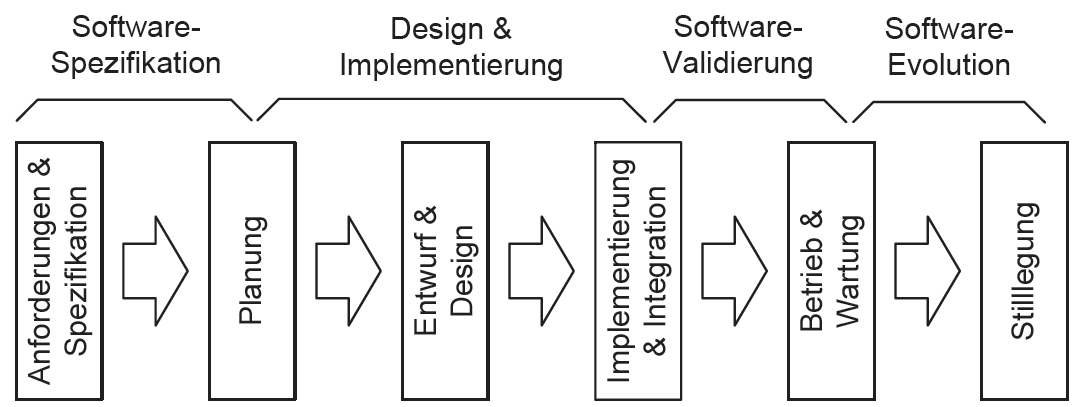
\includegraphics[width=\textwidth,keepaspectratio]{softwarelebenszyklus.PNG}
	\caption{Lebenszyklus eines Softwareprojekts}
	\cite[S.13]{schatten2010}
	\label{img:softwarelebenszyklus}
\end{figure}
\noindent In Abbildung \ref{img:softwarelebenszyklus} lassen sich die wesentlichen Schritte des Software-Lebenszyklus erkennen. Diese sind hier entweder grob in vier Stufen oder differenzierter in sechs Stufen unterteilt. Es gibt keine Vorschriften über die Anzahl oder die Bezeichnungen der Abstufungen, sodass es sehr viele unterschiedliche Versionen des Software-Lebenszyklus und damit Vorgehensmodelle für die Softwareentwicklung gibt. Grundlegende Dinge, die hier durch \textit{Software-Spezifikation}, \textit{Design und Implementierung}, \textit{Software-Validierung} und S\textit{oftware-Evolution} dargestellt werden, "`finden sich [jedoch] nahezu in allen Projekten wieder"' \cite[S.13]{schatten2010}. \\ 
Detaillierter lässt sich der Software-Lebenszyklus in die sechs Phasen \textit{Anforderung und Spezifikation}, \textit{Planung}, \textit{Entwurf und Design}, \textit{Implementierung und Integration}, \textit{Betrieb und Wartung} und \textit{Stilllegung} aufteilen. \\
Die Einteilung eines Softwareprojekts in Phasen "`kann den Entwicklerteams als Leitlinie dienen, um ein Software-Projekt im Team erfolgreich zu strukturieren und abzuwickeln"' \cite[S.11]{schatten2010}. Dabei können die Phasen je nach Vorgehensmodell variieren oder wahrgenommen werden.


\subsection{Vorgehen bei der Beschreibung und Analyse der Anforderungen}
Die Beschreibung und Analyse von Anforderungen ist der erste Schritt bei fast jedem IT-Projekt. Zunächst wird "`aus der in einer systematischen Ermittlung gewonnenen Information [.] bei der Dokumentation eine präzise Anforderungsspezifikation erstellt"' \cite[S.44]{partsch2010}. Das Ziel dabei ist, "`möglichst vollständige Kundenanforderungen in guter Qualität zu dokumentieren und dabei Fehler möglichst frühzeitig zu erkennen und zu beheben"' \cite[S.11]{PohlRupp2015}. Für so eine Anforderungsanalyse gibt es unterschiedliche Methoden, die jedoch alle "`vor allem gesunden Menschenverstand voraus[setzen]"' \cite[S.58]{partsch2010}.\\
Quelle zur Ermittlung der Anforderungen sind Dokumente, bereits existierende Systeme und hauptsächlich die sog. Stakeholder. Diese sind "`Person[en] oder Organisation[en], die (direkt oder indirekt) Einfluss auf die Anforderungen ha[ben]"'\cite[S.21]{PohlRupp2015}. Gemeint sind damit also alle Menschen, die in irgendeiner Weise mit der Software zu tun haben oder haben werden, z.B. der Kunde, der Nutzer, die Entwickler etc. \\
Da der Auftraggeber oft nicht in der Lage ist genau auszudrücken, was er will und braucht, ist es die Aufgabe der Entwickler "`in Software-Projekten frühzeitig mit dem Kunden und den späteren Nutzern [zu] reden, um zu erfahren, was sie sich vorstellen"' \cite[S.15]{kleuker2006}.\\
Es muss also eine ständige Kommunikation und Zusammenarbeit sichergestellt werden. So eine Zusammenarbeit setzt "`ein gewisses Verständnis der Arbeitsabläufe des Kunden, genauer dessen Geschäftsprozesse \cite[vgl.][]{Gad03}, [voraus], die mit der zu entwickelnden Software im Zusammenhang stehen"' \cite[S.15]{kleuker2006}.


\subsection{Qualitätssicherung der Anforderungen}
"`Grundsätzlich gilt, dass die Produkte aller Tätigkeiten bei der Softwareentwicklung [...] qualitätsgesichert [...] werden müssen"' \cite[S.55]{Winter1999}. Deshalb "`ist es notwendig, die Qualität der entwickelnden Anforderungen zu überprüfen"'\cite[S.95]{PohlRupp2015}, um Probleme der Anforderungsermittlung (siehe Kapitel \ref{anforderungen}) zu lösen.  \\
Diese ständige Qualitätssicherung dient dazu, Fehler möglichst früh in dem Softwarelebenszyklus zu erkennen und zu beheben. Der Grund dafür ist, dass die Fehlerbehebung in der Softwareentwicklung mit steigendem Projektfortschritt mehr Aufwand verursacht \cite[vgl.][S.2]{hussmann}. Aufwand kann dabei Geld, Zeit oder auch andere zu erbringende Leistung oder Einsatz sein. Das Ziel ist daher, Fehler schon möglichst früh in dem Projektverlauf zu beseitigen. \\

\noindent Dieser Aufwand der Fehlerbehebung ist der Grund für die Qualitätssicherung der Anforderungsermittlung und dadurch ist sie so wichtig für den Erfolg eines Projektes. Diese wichtige Rolle wird in dem folgenden Balkendiagramm dargestellt:
\begin{figure}[H]
	\hspace{-2cm}
	\centering
	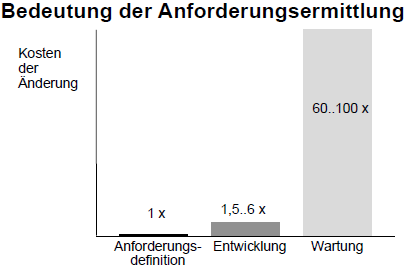
\includegraphics[width=350px,keepaspectratio]{TUDresden.png}
	\caption{Aufwand der Fehlerbehebung in Softwareprojekten}
	\cite[S.2]{hussmann}
	\label{img:TUDresden}
\end{figure}
\noindent Das Diagramm beschreibt den Aufwand der Fehlerbehebung in einem Softwareprojekt in Abhängigkeit von dem Projektfortschritt. Der Fortschritt wird dabei als Phasen des Softwarelebenszyklus dargestellt, wobei dieser vereinfacht nur in Anforderungsdefinition, Entwicklung und Wartung aufgeteilt ist. \\

\noindent Wird ein Fehler in der Phase der Anforderungsermittlung oder am Anfang des Projektes behoben, wird der Aufwand dafür mit dem Faktor Eins multipliziert. Sobald ein Fehler gefunden wurde, gilt es die Anforderung zu überarbeiten und ihn einfach zu korrigieren.\\
Während der Entwicklung des Projektes ist der Aufwand meist um das 1,5 bis 6-fache höher. Grund dafür ist, dass Fehler, die sich dann noch in der Software befinden, oft mehrere Bereiche betreffen und viel verändert und berücksichtigt werden muss bevor man sie entgültig beheben kann.\\
Am meisten Aufwand verursacht die Fehlerbehebung, falls der Fehler erst am Ende des Software-Lebenszyklus entdeckt wird. Dabei ist die Software schon in Betrieb und befindet sich in der Wartung. Um dort einen Fehler zu beheben, müssen oft ganze Programmabschnitte verändert werden, damit die Software wieder fehlerfrei läuft. Es hat also große Folgen, wenn ein Teil des Programmes während der Wartung verändert werden muss, weshalb der Aufwand etwa 60 bis 100 mal höher ist als zu Anfang des Projekts. \\
Deshalb ist es so wichtig, die einzelnen Phasen eines Software-Lebenszyklus sorgfältig zu bearbeiten und zu überprüfen, sodass keine Fehler auftreten oder diese schon so früh wie möglich erkannt werden. Es sollte daher nicht zu früh und unvorbereitet mit der Entwicklung begonnen werden.\\
Obwohl es Ausnahmen gibt, lohnt sich der Aufwand in der Analyse meistens, da "`viele schwerwiegende Fehler in den frühen Phasen IS-Entwicklung [Informationssystem-Entwicklung; Anmerk. d. Verf.] gemacht werden"' \cite[S.316]{Alpar2016}. Trotzdem wird in vielen Fällen zu voreilig mit der Entwicklung angefangen. \\
"Die Analyse der in einer Anforderungsdefinition festgelegten Anforderungen zielt letztlich darauf ab, Aufschluss über die Qualität der Anforderungsbeschreibung zu erhalten"' \cite[S.51]{partsch2010}. Kriterien für die Qualität lassen sich hauptsächlich in Inhalt, Dokumentation und Abgestimmtheit gliedern. Es wird sich also damit befasst, ob die Anforderungen vollständig, detailliert, passend dokumentiert und mit allen Stakeholdern abgestimmt sind. Für jeden der drei Qualitätsaspekte gibt es damit unterschiedliche Prüfkriterien \cite[vgl.][S.97]{PohlRupp2015}.

\subsubsection{Qualitätsaspekt Inhalt}
"`Der Qualitätsaspekt >>Inhalt<< bezieht sich auf die Überprüfung von Anforderungen auf inhaltliche Fehler"' \cite[S.98]{PohlRupp2015}. Dafür gibt es acht Prüfkriterien\cite[vgl.][S.98]{PohlRupp2015}: 
\begin{description}[font=\itshape]\setlength\itemsep{0em}
\item[Vollständigkeit:] Wurden alle relevanten Anforderungen erfasst?
\item[Korrektheit:] Beschreibt jede Anforderung die dafür notwendigen Informationen?
\item[Verfolgbarkeit:] Können die Anforderungen verfolgt, also z.B. auf die Quelle zurückgeführt werden?
\item[Adäquatheit:] Enthalten die Anforderungen die Bedürfnisse und Wünsche der Stakeholder angemessen?
\item[Konsistenz:] Gibt es Widersprüche zwischen den Anforderungen?
\item[Vorzeitige Entwurfsentscheidungen:] Wurden Entwurfentscheidungen vorweggenommen, die nicht durch Randbedingungen bestimmt sind?
\item[Überprüfbarkeit:] Können Abnahme- und Prüfkriterien anhand der Anforderungen definiert werden?
\item[Notwendigkeit:] Trägt jede Anforderung zu dem definierten Ziel bei?
\end{description}

\subsubsection{Qualitätsaspekt Dokumentation}
Bei der Dokumentation geht es darum, die "`Anforderungen auf Mängel in der Dokumentation bzw. auf Verstöße gegen geltende Dokumentationsvorschriften"'\cite[S.99]{PohlRupp2015} zu überprüfen. Hierbei gibt es folgende vier Prüfkriterien\cite[vgl.][S.99f.]{PohlRupp2015}:
\begin{description}[font=\itshape]\setlength\itemsep{0em}
\item[Konformität:] Wurden die Anforderungen in dem vorgeschriebenen Dokumentationsformat strukturiert und in der richtigen Modellierungssprache dokumentiert?
\item[Verständlichkeit:] Können die Anforderungen in dem gegebenen Kontext ggf. mithilfe eines Glossars verstanden werden?
\item[Eindeutigkeit:] Ist eine eindeutige Interpretation möglich?
\item[Konfirmität mit Dokumentationsregeln:] Sind vorgegebene Dokumentationsregeln und -richtlinien eingehalten worden?
\end{description}

\subsubsection{Qualitätsaspekt Abgestimmtheit}
Die Abgestimmtheit stellt sicher, dass keine "'Mängel in der Abstimmung der Anforderungen unter relevanten Stakeholdern"'\cite[S.100]{PohlRupp2015} vorliegen. Auch hierbei gibt es folgende drei Prüfkriterien\cite[vgl.][S.100]{PohlRupp2015} :
\begin{description}[font=\itshape]\setlength\itemsep{0em}
\item[Abstimmung:] Wurde jede Anforderung mit relevanten Stakeholdern abgestimmt?
\item[Abstimmung nach Änderungen:] Wurde jede Änderung der Anforderungen auch abgestimmt?
\item[Konflikte:] Wurden alle bekannten Konflikte gelöst?
\end{description}

\subsection{Anforderungskategorisierung}
Anforderungen werden kategorisiert und nach Wichtigkeit eingeteilt. Das ist hilfreich, da die Anforderungen unterschiedlich zur Zufriedenheit der Stakeholder beitragen \cite[vgl. S.24]{PohlRupp2015}. Durch Kategorisierung lassen sie sich leichter einordnen, um Aufwand und Priorität besser abschätzen zu können. \\
In diesem Fall werden die Anforderungen nach dem Kano-Modell kategorisiert. Demnach gibt es drei Kategorien \cite[vgl. S.24]{PohlRupp2015}:
\begin{description} 
\item[Basisfaktoren] sind selbstverständliche unterbewusste Systemmerkmale, die vorausgesetzt werden. 
\item[Leistungsfaktoren] sind bewusste, explizit geforderte Systemmerkmale.
\item[Begeisterungsfaktoren] sind für den Stakeholder unbekannte Systemmerkmale, die er während der Benutzung als angenehme Überraschung entdeckt.
\end{description}
Mit der Zeit werden aus Begeisterungsfaktoren Leistungsfaktoren und aus Leistungsfaktoren Basisfaktoren, da der Nutzer sich an die Merkmale gewöhnt und sie irgendwann voraussetzt. Das Modell lässt sich grafisch darstellen: 

\begin{figure}[H]
	\centering
	\includegraphics{kano.pdf}
	\caption{Grafische Darstellung des Kano-Modells}
	\cite[S.25]{PohlRupp2015}
	\label{img:kano}
\end{figure}
\noindent Die Grafik zeigt die Zufriedenheit der Stakeholder in Abhängigkeit von dem Erfüllungsgrad der jeweiligen Faktoren. Auf einer dritten Achse wird die Zeit dargestellt, wodurch die Anforderungen die Kategorien wechseln können. \\
Die Basisfaktoren müssen erfüllt sein, um eine massive Unzufriedenheit der Stakeholder zu vermeiden \cite[vgl. S.106]{Kano}. Sie werden vorrausgesetzt und haben daher nur den Nutzen, Unzufriedenheit zu vermeiden. Daher verläuft die Funtkion negativ exponentiell. \\
Die Funktion der Leistungsfaktoren verläuft linear und schneidet den Nullpunkt. Diese Faktoren erzeugen proportional Unzufriedenheit, wenn sie nicht erfüllt sind, und Zufriedenheit, wenn sie erfüllt sind \cite[vgl. S.106]{Kano}. \\
Da die Begeisterungsfaktoren vorher den Stakeholdern nicht bekannt sind, kann ihr unzureichender Erfüllungsgrad keine Unzufriedenheit verursachen, da sie nicht erwartet werden oder bekannt sind \cite[vgl. S.106]{Kano}. Das Vorhandensein dieser Faktoren freut jedoch die Stakeholder, wodurch es zu einem überproportionalen Nutzen bei steigender Erfüllung kommt. Deshalb ist die Funktion der Begeisterungsfaktoren linear und erreicht niemals den Wert null oder weniger, aber steigt sehr schnell an. \\

\noindent Es ist ungeklärt, ob man diese Faktoren und ihre Eigenschaften so auf die Anforderungen bei der Erstellung eines Prototyps anwenden kann. Laut Pombergers Definition soll ein explorativer Prototyp ermöglichen, die Vorstellungen der Anwender "`anhand von Anwendungsbeispielen zu prüfen und die gewünschte Funktionalität zu ermitteln"' \cite[S.27]{pomberger2004}, es soll also die Analyse und die Anforderungsspezifikation unterstützen. Das bedeutet, dass der Prototyp nicht alle Anforderungen enthalten kann, besonders die Leistungs- und Begeisterungsfaktoren nicht, und genau im Gegenteil dazu dient, Anforderungen zu ermitteln. \\
Kanos Begeisterungsfaktoren widersprechen zudem dem weit verbreiteten Vorgehen bei einer erfolgreichen Anforderungsanalyse. Wie von Pohl und Rupp beschrieben ist dafür "`eine gute Kommunikation und [...] Qualität der Zusammenarbeit mit den Stakeholdern"' \cite[S.33]{PohlRupp2015} notwendig, um ihn "`erfolgreich in den Ermittlungsprozess einzubinden"' \cite[S.34]{PohlRupp2015}. Durch diese enge Zusammenarbeit werden alle Anforderungen abgesprochen, sodass es keine Begeisterungsfaktoren mehr geben kann.


\subsection{Abgrenzung des Systems und Systemkontextes}
Die Abgrenzung eines Systemes zu seiner umgebung und zu den Schnittstellen ist essentiell für den Entwurf eines korrekten Produktes. Dafür müssen die System- und Kontextgrenzen bestimmt werden. \\
Dadurch wird Aufwand vermieden, indem bereits vorhandene Funktionen evtl. integriert oder nur in etwas abgeänderter Weise übernommen werden. Außerdem bringt sie Klarheit über die Arten der Informationsgewinnung und -weiterverarbeitung, um Missverständnisse zu vermeiden. Es ist wichtig, "`die Grenzen des Systems zum Systemkontext und die Grenzen des Systemkontexts zur irrelevanten Umgebung zu bestimmen"' \cite[S.20]{PohlRupp2015}, da der Systemkontext "`auch die Anforderungen an das zu entwickelnde System bestimmt"' \cite[S.20]{PohlRupp2015}. \\
Der praktische Teil zu diesem Kapitel fällt weg, da diese Arbeit \ac{COC} als Grundlage nutzt und Systemgrenzen und -schnittstellen daher schon klar definiert sind. 

\subsection{Arten und Ziele des Prototypings}
Prototyping beschreibt "`eine Vorgehensweise bei der Softwareentwicklung, bei der nicht sofort ein endgültiges Softwaresystem, sondern zunächst ein oder mehrere Prototypen erstellt werden"' \cite[S.152]{gabler}. Dabei wird nach Kuhrmann zwischen horizontalem und vertikalem Prototyping unterschieden \cite[vgl.][]{Kuhrmann2012}: \\ 
\textbf{Horizontales Prototyping} bezieht sich auf einen bestimmten Bereich der Software, z.B. die Benutzeroberfläche. Der Bezug zu der technischen Funktionalität und der tatsächlichen Implementierung ist dabei nicht gegeben. Nur die eine Ebene des Programms soll vorgestellt werden.\\
Beim \textbf{vertikalen Prototyping} wird ein Ausschnitt komplett in allen Ebenen vollständig implementiert. Diese Art dient zur Demonstration von komplexer Funktionalität.\\

\noindent Darüber hinaus unterscheidet die IEEE das Prototyping anhand von Anwendungszwecken \cite[vgl.][S.826]{ieeeprot}: 
\begin{description}
\item[Exploratives Prototyping] wird benutzt, wenn man das Problem und die Anforderungen noch nicht genau kennt. Indem viele Ideen und Ansätze ausprobiert werden, lernt der Entwickler die Arbeit und die Anforderungen des Kunden besser kennen, um die Anforderungen zu identifizieren.
\item[Experimentelles Prototyping] zielt auf das Sammeln von Erfahrungen und Ideen. Der Anwender kann mit dem Prototypen experimentieren, um Ideen an das Programm weiterzuentwickeln und Anforderungen zu konkretisieren. Währenddessen enthält der Entwickler Eindrücke von der Realisierbarkeit des Systems und technischen Herausforderungen.
\item[Evolutionäres Prototyping] stellt die Softwareentwicklung nicht als ein temporäres Projekt, sondern als eine fortlaufende Entwicklung dar. Dabei wird das Programm nach und nach erweitert, wobei der Entwickler eng an der Seite des Anwenders das System immer weiter erweitert.
\end{description}
Die Definition des evolutionären Prototypings widerspricht jedoch der allgemeinen Definition nach \cite{gabler}. Das Ergebnis des explorativen und des experimentellen Prototypings ist ein Prototyp im engeren Sinne, der der Demonstration dient. Dieser wird nach der Erfüllung seiner Aufgaben nicht mehr benötigt \cite[vgl.][S.21]{liggesmeyer2012}. Beim evolutionären Prototyping hingegen entsteht ein Pilotsystem, das der Kern des Produktes ist. Der Prototyp wird also fließend zum laufenden Produkt \cite[vgl.][S.24]{liggesmeyer2012} und ist damit eigentlich kein Prototyp laut Definition mehr.

\newpage

\section {Istanalyse}

\subsection{Bestandsrechnung in Compas Cockpit} \label{bestandsrechnung}
Der aktuelle Algorithmus für die Bestandsrechnung in \ac{COC} ermittelt zuerst den Bruttobestand der Besatzungen \cite[vgl.][S.8]{capfunc}. 
Dazu wird der aktuelle Pilotenbestand mit allen Formen von Zu- und Abgängen z.B. durch Umschulungen, Altersabgänge oder Neueinstellungen und Kündigungen sowie allen bezahlungswirksamen Fehlzeiten wie Teilzeit, Mutterschutz oder Fluguntauglichkeit errechnet \cite[vgl.][S.19]{benutzerhandbuch}. Insgesamt gibt es 16 Kategorien, die hier aber der Übersicht halber nicht alle genannt werden. \\
Von diesem Bruttobestand werden alle weiteren Fehlzeiten, die sich grob in Urlaub und Krankheit einteilen lassen, subtrahiert, was zu dem Nettobestand führt \cite[vgl.][S.8]{capfunc}. \\
Das Ergebnis aller verfügbaren Piloten ergibt sich dann durch die Subtraktion von freien Tagen, die den Piloten zustehen. Auch die Arten und die Berechnung der freien Tage werden hier nicht weiter erläutert. \\
Dadurch ergibt sich der Bestand aller verfügbaren Piloten in \ac{BT}. Diese \acp{BT} lassen sich auf Tages-, Wochen- und Monatsbasis darstellen und zusammenfassen. 


\subsection{Anforderungsanalyse- und kategorisierung}
Die Planerinnen formulierten folgende Anforderungen \cite[vgl.]{Gespraech2}:
\begin{description}
\item Basisfaktoren: Es soll ein Programm erstellt werden, dass die Kapazitäts- und später auch die Schulungsplanung automatisch regelt. Dafür müssen vor allem die Gruppen und Untergruppen eingeteilt und dargestellt werden können. Der Zeitraum soll 15 Monate betragen, um die Urlaubsplanung des jeweils kommenden Jahres mit einfließen lassen zu können. Eine Bestandsrechnung wird also benötigt, die später um die Bedarfsrechnung ergänzt werden soll. Das Programm wird dann nach und nach erweitert bis es in etwa den Funktionalitäten von \ac{COC} entspricht. \\
Der Kunde legt außerdem viel Wert auf Nachvollziehbarkeit. Es soll bei jeder Zelle der Tabellen verstanden werden können, woher die Daten her kommen oder wie sie berechnet werden. Dazu soll es wie bei \ac{COC} die Möglichkeit geben, Reports für einzelne bestimmte Daten abfragen zu können.
\item Leistungsfaktoren: Da es sich um den Entwurf eines Prototyps zur Kapazitätsplanung handelt, ist die Schulungsplanung ein Leistungsfaktor. Dazu gehören auch Bewerbungen für Schulungen. Ein weiterer Leistungsfaktor ist die Bedarfsrechnung. Diese Leistungsfaktoren werden aber später ergänzt, sodass sie nicht Bestandeil dieses Lösungsentwurfs sind. \\
Darüber hinaus wird eine gute Performance erwartet, um die Planung zu erleichtern und Zeit zu sparen.
\item Begeisterungsfaktoren: Modernes Design ist einer der Begeisterungsfaktoren. Dabei ist wünschenswert, das Programm so zu designen, dass sich Cockpit- und Kabinenplaner/innen ersetzen können und die Bedienung und Anordnung der Elemente gleich ist. 
\end{description}
Da sich diese Arbeit aber nur mit der Entwicklung eines Lösungsentwurfs für den Prototypen beschäftigt, stehen die Basisfaktoren im Vordergrund. Die Leistungs- und Begeisterungsfaktoren sind für einen explorativen Prototypen erst einmal nur optional. Sie kommen im Verlauf des Projektes dazu. Trotzdem ist eine Bestimmung davon wichtig, um das System abzugrenzen und Schwerpunkte festzulegen.

\subsection {Die Schnittstelle: Das Crew Management System}
Die Quelle, aus der \ac{COC} die benötigten Daten entnimmt, ist das \ac{CMS} oder genauer gesagt die \ac{CDB}. Unter dem \ac{CMS} wird das gesamte Planungssystem der Lufthansa verstanden, das aus vielen verschiedenen Systemen besteht. Im Mittelpunkt davon steht die \ac{CDB}, wo die Daten zusammen fließen und in der Datenbank gespeichert werden. Es wird also von sehr vielen Seiten aus auf die \ac{CDB} zugegriffen, was ihr sehr viel Leistung und Performance abverlangt. \\
Damit \ac{COC} alle benötigten Daten in der tagesgenauer Form erhalten kann, bereitet die \ac{CDB} diese Daten zwei mal im Monat auf, indem sie sie aus allen anderen Tabellen anderer Systeme herausfiltert und dann Views erstellt, die der benötigten Form entspricht. Das Erstellen dieser View verursacht dabei sehr viel Aufwand und Auslastung der \ac{CDB}.\\
Wenn über \ac{COC} die aktuellen Daten dann angefordert werden, werden sie in die eigene Compas-Datenbank geladen, wo direkt drauf zugegriffen werden kann. Das Aktualisieren der Tabellen aus der View nimmt dabei nicht viel Zeit in Anspruch, da die Daten nur geladen und nicht verändert oder formatiert werden müssen.


\section [Konkrete Modernisierung und Anpassung von Compas Cockpit]{Konkrete Modernisierung und Anpassung von \\ Compas Cockpit}
\subsection{Veränderungen bei der Datenaufbereitung}
Um Laufzeit- und Performanceprobleme bei der Datenaufbereitung zu vermeiden, wird eine andere Vorgehensweise als in \ac{COC} benötigt. Die erste und einfachste Idee dazu ist, alle Rohdaten, welche zur Erstellung der Views verwendet werden, unverändert von der \ac{CDB} in die Compas-Datenbank zu laden und dort dann die Views zu erstellen \cite[vgl. dazu][]{Gespraech5}. \\
Dadurch hat die \ac{CDB} nur noch die Aufgabe, die Tabellen der Rohdaten zur Verfügung zu stellen, und es wird ihr keine große Leistung abverlangt. Die Auslastung wird von der \ac{CDB} auf die Compas-Datenbank verschoben. Da diese Datenbank aber von keinen anderen Systemen genutzt wird, ist es dort kein Problem, wenn sie für längere Zeit ausgelastet wird, um die Daten aufzubereiten. Solange kein Compas-Nutzer auf die Datenbank zugreifen will, können dort also die Views z.B. am Wochenende erstellt werden. \\
Diese Idee kann aber aufgrund rechtlicher Vorschriften nicht umgesetzt werden. Bei der Datenaufbereitung wird mit personenbezogenen Daten gearbeitet \cite[vgl.][S.6]{CMS}, auch wenn diese später nicht in den Views gefunden werden können. Die Views enthalten also keine personenbezogenen Daten, für ihre Erstellung sind sie aber notwendig. Da "`bei der Verarbeitung personenbezogener Daten [.] die Bestimmungen des Bundesdatenschutzgesetzes zu berücksichtigen"' \cite[S.6]{CMS} sind, dürfen diese nicht auf der Compas-Datenbank liegen. Außerdem wurden weitere "`spezielle Schutzvorschriften zwischen den Geschäftsleitungen und den Mitarbeitervertretungen [der Lufthansa AG; Anmerk. d. Verf.] definiert"' \cite[S.6]{CMS}. Es ist deshalb nicht möglich, die Daten dort ohne eine Genehmigung zu formatieren.

\subsection{Veränderungen in der Bestandsrechnung}
In der in Kapitel \ref{bestandsrechnung} beschriebenen Bestandsrechnung von \ac{COC} müssen einige Zeilen angepasst werden, damit sie der bisherigen Bestandsrechnung der Kabine entspricht. Diese Anpassung wurde mit dem Kunden genau besprochen \cite[vgl.][]{bestanddet}. \\
Einige Zeilen wie "`Verlängerer Teilzeit"' oder "`Alterssonderurlaub"' fallen weg, da so etwas bei der Kabinenbesatzung nicht vorkommen kann. Eine Änderung wird für das Feld "`Umschulungen"' benötigt, die in \ac{COC} einfach verrechnet wurden. In \ac{CAB} ist es notwendig, zwischen Schulungen, die kürzer als fünf Tage, und welchen, die mindestens fünf Tage dauern zu unterscheiden, weshalb zwei Zeilen für die beiden Arten der Schulungen benötigt werden. \\ %Wieso?
Auch das Feld "`FO-Leistung gesamt"' muss angepasst werden. Die Vorgehensweise in \ac{COC} ist, dass Umschüler bereits zu Beginn einer Schulung auf eine neue \ac{PU} zu dieser \ac{PU} zählen und die Flugstunden während der Schulung schon als FO-Leistung zu dem verfügbaren Bestand addiert werden. Bei der Kabinenbesatzung zählt eine Person erst zu der neuen \ac{KG}, wenn sie die Schulung beendet hat, leistet aber während der Schulung auch schon Flugstunden für die neue \ac{KG}. \\%Lösung dafür?
Bei der restlichen Bestandsrechnung kann genau so vorgegangen werden, wie es bereits in \ac{COC} für die Cockpit-Mitarbeiter implementiert ist.

%\subsection{Prämissen der Bestandsrechnung}

\subsection{Abbilden der Mehrfachqualifikationen und Einbindung der Kleingruppen}
Nach Absprache des Problems der Mehrfachqualifikationen mit dem Fachbereich haben sich die Anforderungen geändert \cite[vgl.][]{Gespraech4}: \\
Die Anwender haben eine Liste von \acp{PU} erstellt, die wie in \ac{COC} aufgebaut sind, mit dem Unterschied, dass die \acp{PU} mehrere Muster besitzen können. Sie stellen es sich so vor, dass die fest eingeteilten \acp{KG} jeweils manuell einer \ac{PU} vom Nutzer zugeordnet werden können. Diese Zuteilung muss natürlich veränderbar und flexibel sein. \\
Deshalb muss anstatt einer direkten Verbindung zwischen einer Person und einer \ac{PU} ein Zwischenschritt mit den \acp{KG} eingebaut werden. Die personalisierte tagesgenaue View enthält also eine Referenz mit der \ac{KG}, in der sich die Person befindet. Danach ist eine neue Tabelle notwendig, wo die \acp{KG} den \acp{PU} zugeordnet werden, die vom Anwender bearbeitet werden kann. Eine \ac{KG} hat damit Bezug zu maximal einer \ac{PU}. \\
%Lösung wie die Qualifikationen in die PUs einfließen

\newpage

\section {Zusammenfassung und Ausblick}
\newpage

\pagenumbering{gobble}
\addcontentsline{toc}{section}{Literaturverzeichnis}
\bibliographystyle{natdin}

\bibliography{literatur}


\newpage

\pagenumbering{Roman}
\setcounter{page}{4}
\section* {Glossar}
\addcontentsline{toc}{section}{Glossar}

\begin{table}[]
\begin{tabular}{l|p{13cm}}
\textbf{Begriff} & \textbf{Erläuterung} \\\hline
Bestandsrechnung & Berechnung des verfügbaren Bestands in Beschäftigungstagen; dieser wird aus dem Bruttobestand und verschiedenen Ab- und Zugängen errechnet\\
Compas Cabin & Gefordertes Programm; soll in Compas Cockpit integriert werden und die Kapazitäts- und Schulungsplanung der Kabinencrew automatisieren\\
Compas Cockpit & Programm zur Kapazitäts- und Schulungsplanung der Cockpit-Mitarbeiter; für die Lufthansa von Lufthansa Systems 1999 entwickelt und seitdem ständig erweitert\\
Crew Database & Zentrale Datenbank der Lufthansa mit Schnittstellen zu vielen unterschiedlichen Systemen; stellt die erforderlichen Daten für Compas zusammen\\
Crew Management System & Überbegriff für alle Schnittstellen-Systeme der Lufthansa mit der Crew Database im Mittelpunkt\\
Deltarechnung & Der Bestand wird ins Verhältnis zum Bedarf gesetzt und daraus das Delta ermittelt\\
Funktion & auch Function; Rolle und Aufgaben, die Piloten oder die Kabinenbesatzung auf einem Flug übernehmen \\
Homebase & Flughafen an dem eine Person oder Gruppe stationiert ist \\  
IEEE & Institute of Electrical and Electronics Engineers; Berufsverband von Igenieuren aus Elektro- und Informationstechnik \\
Kapazitätsplanung & Mithilfe der Deltarechnung sollen dabei die richtige Anzahl an Personen mit den richtigen Qualifikationen zum richtigen Zeitpunkt verfügbar sein\\
Kleingruppe & Gruppen für die Kap.- und Schulungsplanung der Kabinenebesatzung; definiert durch  Funktion, Homebase, Unterfunktion, Fluggesellschaft und Flugzeugtyp(en)\\
NetLine/Crew & Von Lufthansa Systems entwickeltes Programm, das alle Phasen des Crewmanagements unterstützt\\
Planungseinheit & auch Planningunit; Gruppen für die Kap.- und Schulungsplanung des Cockpits; definiert durch Flugzeugtyp, Funktion, Homebase, Fluggesellschaft, Unterfunktion\\
Report & Detailabfrage in Compas Cockpit, wo Planzahlen aufbereitet und detaillierter als in der Gesamtübersicht dargestellt werden\\
Unterfunktion & auch Subfunction; optionale Erweiterung der Funktion \\

\end{tabular}
\end{table}
\newpage

\section* {Anlagenverzeichnis}
\addcontentsline{toc}{section}{Anhang}
\newpage

\end{document}

